\documentclass[11pt]{article}\usepackage[]{graphicx}\usepackage[]{color}
%% maxwidth is the original width if it is less than linewidth
%% otherwise use linewidth (to make sure the graphics do not exceed the margin)
\makeatletter
\def\maxwidth{ %
  \ifdim\Gin@nat@width>\linewidth
    \linewidth
  \else
    \Gin@nat@width
  \fi
}
\makeatother

\definecolor{fgcolor}{rgb}{0.345, 0.345, 0.345}
\newcommand{\hlnum}[1]{\textcolor[rgb]{0.686,0.059,0.569}{#1}}%
\newcommand{\hlstr}[1]{\textcolor[rgb]{0.192,0.494,0.8}{#1}}%
\newcommand{\hlcom}[1]{\textcolor[rgb]{0.678,0.584,0.686}{\textit{#1}}}%
\newcommand{\hlopt}[1]{\textcolor[rgb]{0,0,0}{#1}}%
\newcommand{\hlstd}[1]{\textcolor[rgb]{0.345,0.345,0.345}{#1}}%
\newcommand{\hlkwa}[1]{\textcolor[rgb]{0.161,0.373,0.58}{\textbf{#1}}}%
\newcommand{\hlkwb}[1]{\textcolor[rgb]{0.69,0.353,0.396}{#1}}%
\newcommand{\hlkwc}[1]{\textcolor[rgb]{0.333,0.667,0.333}{#1}}%
\newcommand{\hlkwd}[1]{\textcolor[rgb]{0.737,0.353,0.396}{\textbf{#1}}}%

\usepackage{framed}
\makeatletter
\newenvironment{kframe}{%
 \def\at@end@of@kframe{}%
 \ifinner\ifhmode%
  \def\at@end@of@kframe{\end{minipage}}%
  \begin{minipage}{\columnwidth}%
 \fi\fi%
 \def\FrameCommand##1{\hskip\@totalleftmargin \hskip-\fboxsep
 \colorbox{shadecolor}{##1}\hskip-\fboxsep
     % There is no \\@totalrightmargin, so:
     \hskip-\linewidth \hskip-\@totalleftmargin \hskip\columnwidth}%
 \MakeFramed {\advance\hsize-\width
   \@totalleftmargin\z@ \linewidth\hsize
   \@setminipage}}%
 {\par\unskip\endMakeFramed%
 \at@end@of@kframe}
\makeatother

\definecolor{shadecolor}{rgb}{.97, .97, .97}
\definecolor{messagecolor}{rgb}{0, 0, 0}
\definecolor{warningcolor}{rgb}{1, 0, 1}
\definecolor{errorcolor}{rgb}{1, 0, 0}
\newenvironment{knitrout}{}{} % an empty environment to be redefined in TeX

\usepackage{alltt}
\usepackage{amsmath}
\usepackage{fullpage}
\usepackage{float}
\usepackage{graphicx}

\title{USVAR: An Implementation of Under-identified SVAR Model}
\author{Jay Raol \and Bin Yang}
\date{\today}
\IfFileExists{upquote.sty}{\usepackage{upquote}}{}
\begin{document}
\maketitle

\abstract{}

\section{Introduction}

\section{Mathematical Model}
For a $m \times 1$ vector of variables, we can define the Structural VAR(SVAR) Model with $p$ lags, in its reduced form, as the following

\begin{equation} \label{eq1}
Y_t = \mathbf{B_1} Y_{t-1} + \mathbf{B_2} Y_{t-2} + \ldots + \mathbf{B_p} Y_{t-p} + u_t, \mathbf{E} [u_t u_t^{'}] = \mathbf{\Sigma} ,
\end{equation}
\\
where $B_{k}$ are the coefficient matrices for $k = 1, \ldots, p$, and $u_t$ is the time $t$ error with covariance matrix $\mathbf{\Sigma}$. Structral shocks $\varepsilon_{t}$ to the reduced form error $u_t$ are often assumed to be related in the following way:

\begin{equation}
u_t = \mathbf{Z} \varepsilon_{t},  \mathbf{E} [\varepsilon_{t} \varepsilon_{t}^{'}] = \mathbf{I}_m,  \mathbf{Z}\mathbf{Z}^{'} = \mathbf{\Sigma}
\end{equation}
\\
We define $\mathbf{Z}$ to be the short-run impact matrix. The SVAR model described in \ref{eq1} and use sign restrictions to determine those appropriate $\mathbf{Z}$s among infinitely many $\mathbf{Z}$s that satisfy the condition $\mathbf{Z} \mathbf{Z}^{'} = \mathbf{\Sigma}$.

\section{Methods and Functions}
  \subsection{Overview}
  
  \subsection{Impulse Responses}
  
  \subsection{Historical Decompositions of Model Errors}
  
\section{Example}
\subsection{Data}
In this section, we demonstrate the use of functions by estimating a model on the data set from Smets \& Wouters (2007), and we try to replicate the results in the first example given in Binning (2013). The author used variables including interest rate, GDP growth, CPI inflation, hours worked, and wage inflation. The author attempts to identify the following shocks: the monetary policy shock, the aggregate demand shock, the aggregate supply shock, the wage mark-up shock and a shock that is left unidentified. In particular, the author uses the following identification scheme:

\begin{center}
$f(\mathbf{Z},\mathbf{B})$ = \bordermatrix{
~   & \varepsilon^{MP} & \varepsilon^{AD} & \varepsilon^{AS} & \varepsilon^{WM} & \varepsilon^{U} \cr
i_0 & + & + & - & - & \times \cr
\Delta log(Y_0) & - & + & + & + & \times \cr
\pi_0 & - & + & - & - & \times \cr
H_0 & \times & \times & \times & + & \times \cr
\Delta log(W_0) & \times & \times & \times & - & \times \cr
i_\infty & \times & \times & \times & \times & \times \cr
\Delta log(Y_\infty) & 0 & 0 & \times & 0 & 0 \cr
\pi_\infty & \times & \times & \times & \times & \times \cr
H_\infty & \times & \times & \times & \times & \times \cr
\Delta log(W_\infty) & \times & \times & \times & \times & \times \cr}
\end{center}

\subsection{Impulse Response}
Given the estimated model from author that uses OLS with lag 2 which has the lowest BIC, we can obtain the impulse response by using the function \textit{usvar}. The following plot is a impulse response plot of all the variables against different shocks with $t_{0}$ at Jan 1996.

\begin{figure}[H]
\centering
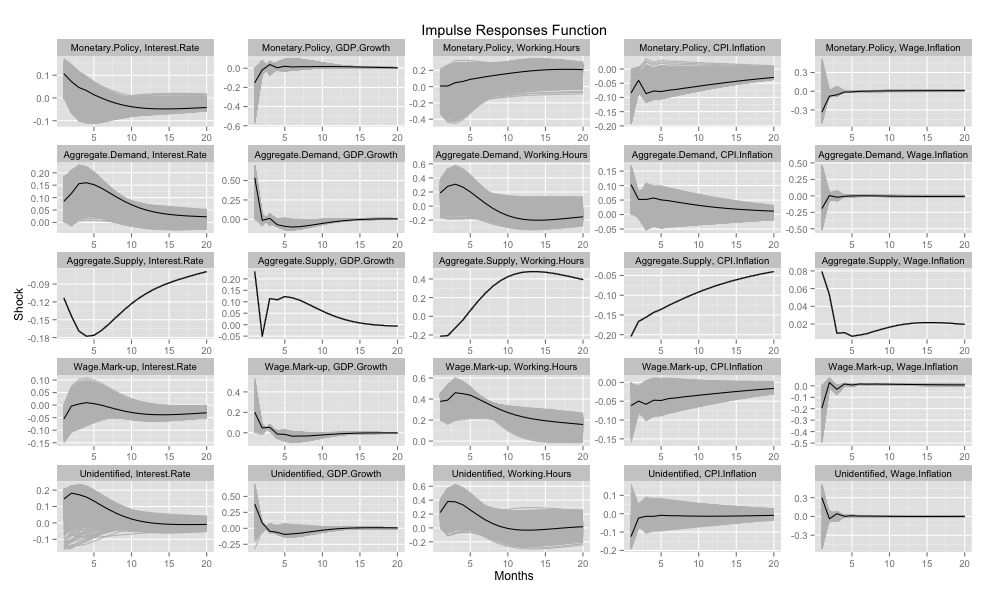
\includegraphics[scale=0.5]{IRF}
\caption{Impulse Response Functions}
\end{figure}





\subsection{Historical Decompostions}

\section{Conclusion}

\bibliography{}

\end{document}
